\documentclass{article}
\usepackage{amsmath}
\usepackage{amssymb}
\usepackage{array}
\usepackage{booktabs}
\usepackage{textcomp}
\usepackage{graphicx}
\usepackage{tikz}
\usepackage{graphics}

\usepackage{amsthm}
\newtheorem{theorem}{Theorem}[section]

\newtheorem{lemma}[theorem]{Lemma}



\newcommand{\coNP}{\textrm{co-}\mathbb{NP}}

\title{hw2}
\author{Ian Chi}
\date{\today}
\begin{document}
\maketitle
\section{}

\begin{enumerate}
    \item 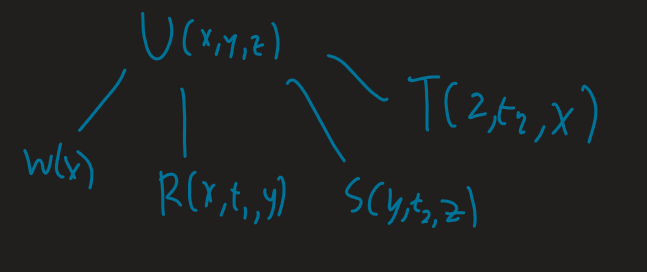
\includegraphics[width=1.0\textwidth]{1a.png}
    \item \(S,R,T\) form a cycle. \(S,R \) contain \(z\). \(R,T\) contain \(u\). \(T,S\) contain \(x\), this forms a cycle.
    \item 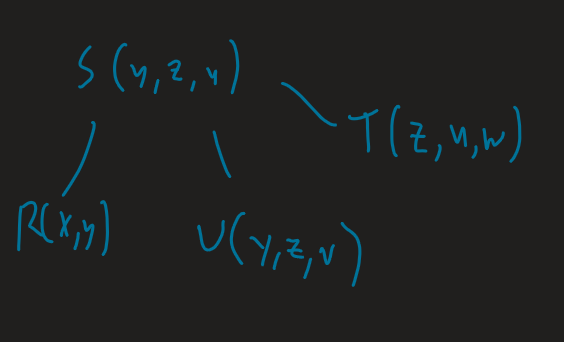
\includegraphics[width=1.0\textwidth]{1c.png}
\end{enumerate}

\newpage
\section{}
\begin{enumerate}
    \item 
    \begin{verbatim}
    SELECT COUNT(*)
    FROM edges e1
    JOIN edges e2 ON e1.dst = e2.src
    JOIN edges e3 ON e2.dst = e3.src
    JOIN edges e4 ON e3.dst = e4.src
    JOIN edges e5 ON e4.dst = e5.src
    WHERE e1.src % 100 = 0
        AND e5.dst % 100 = 0;
    \end{verbatim}
    it took 3:19 for the full graph

    \item
    E(x,y) - E(y,z) - E(z,w) - E(w,u) - E(u,v)
    \item 
    \begin{verbatim}
        WITH
        E1 AS (SELECT * FROM edges WHERE src % 100 = 0),
        E5 AS (SELECT * FROM edges WHERE dst % 100 = 0),

        E4b AS (SELECT * FROM edges WHERE dst IN (SELECT src FROM E5)),
        E3b AS (SELECT * FROM edges WHERE dst IN (SELECT src FROM E4b)),
        E2b AS (SELECT * FROM edges WHERE dst IN (SELECT src FROM E3b)),
        E1b AS (SELECT * FROM E1 WHERE dst IN (SELECT src FROM E2b)),

        E2t AS (SELECT * FROM E2b WHERE src IN (SELECT dst FROM E1b)),
        E3t AS (SELECT * FROM E3b WHERE src IN (SELECT dst FROM E2t)),
        E4t AS (SELECT * FROM E4b WHERE src IN (SELECT dst FROM E3t)),
        E5t AS (SELECT * FROM E5 WHERE src IN (SELECT dst FROM E4t))

        SELECT COUNT(*)
        FROM E1b e1
        JOIN E2t e2 ON e1.dst = e2.src
        JOIN E3t e3 ON e2.dst = e3.src
        JOIN E4t e4 ON e3.dst = e4.src
        JOIN E5t e5 ON e4.dst = e5.src;

    \end{verbatim}
    \item Time: 177973.167 ms (02:57.973)
    the time maybe is saved a tiny  bit but pgsql probably already does some optimization

\end{enumerate}

\section{}

\begin{enumerate}
    \item 
    \begin{verbatim}
        for each z:
            count_z[z] = number of tuples (z, u) in E3

        for each y:
            count_y[y] = 0
            for each (y, z) in E2 with this y:
                count_y[y] += count_z[z]

        total = 0
        for each (x, y) in E1:
            total += count_y[y]

        output total
    \end{verbatim}
    \item 
    \begin{verbatim}
        WITH
        z_count AS (
            SELECT src AS z, COUNT(*) AS cz
            FROM edges
            GROUP BY src
        ),

        y_count AS (
            SELECT e.src AS y, SUM(zc.cz) AS cy
            FROM edges e
            JOIN z_count zc ON e.dst = zc.z
            GROUP BY e.src
        )

        SELECT SUM(yc.cy) AS path_count
        FROM edges e
        JOIN y_count yc ON e.dst = yc.y;

    \end{verbatim}
    \item Time: 316.340 ms vs Time: 177832.565 ms (02:57.833)

\end{enumerate}



\end{document}